% Created 2024-04-28 Sun 20:49
% Intended LaTeX compiler: xelatex
\RequirePackage{fix-cm}
\PassOptionsToPackage{svgnames}{xcolor}
\documentclass[11pt]{article}
\usepackage{fontspec}
\usepackage{sectsty}
\allsectionsfont{\sffamily}
\usepackage{enumitem}
\setlist[description]{style=unboxed,font=\sffamily\bfseries}
\usepackage{listings}
\lstset{frame=single,aboveskip=1em,
	framesep=.5em,backgroundcolor=\color{AliceBlue},
	rulecolor=\color{LightSteelBlue},framerule=1pt}
\usepackage{xcolor}
\newcommand\basicdefault[1]{\scriptsize\color{Black}\ttfamily#1}
\lstset{basicstyle=\basicdefault{\spaceskip1em}}
\lstset{literate=
	    {§}{{\S}}1
	    {©}{{\raisebox{.125ex}{\copyright}\enspace}}1
	    {«}{{\guillemotleft}}1
	    {»}{{\guillemotright}}1
	    {Á}{{\'A}}1
	    {Ä}{{\"A}}1
	    {É}{{\'E}}1
	    {Í}{{\'I}}1
	    {Ó}{{\'O}}1
	    {Ö}{{\"O}}1
	    {Ú}{{\'U}}1
	    {Ü}{{\"U}}1
	    {ß}{{\ss}}2
	    {à}{{\`a}}1
	    {á}{{\'a}}1
	    {ä}{{\"a}}1
	    {é}{{\'e}}1
	    {í}{{\'i}}1
	    {ó}{{\'o}}1
	    {ö}{{\"o}}1
	    {ú}{{\'u}}1
	    {ü}{{\"u}}1
	    {¹}{{\textsuperscript1}}1
            {²}{{\textsuperscript2}}1
            {³}{{\textsuperscript3}}1
	    {ı}{{\i}}1
	    {—}{{---}}1
	    {’}{{'}}1
	    {…}{{\dots}}1
            {⮠}{{$\hookleftarrow$}}1
	    {␣}{{\textvisiblespace}}1,
	    keywordstyle=\color{DarkGreen}\bfseries,
	    identifierstyle=\color{DarkRed},
	    commentstyle=\color{Gray}\upshape,
	    stringstyle=\color{DarkBlue}\upshape,
	    emphstyle=\color{Chocolate}\upshape,
	    showstringspaces=false,
	    columns=fullflexible,
	    keepspaces=true}
\usepackage[a4paper,margin=1in,left=1.5in]{geometry}
\usepackage{parskip}
\makeatletter
\renewcommand{\maketitle}{%
  \begingroup\parindent0pt
  \sffamily
  \Huge{\bfseries\@title}\par\bigskip
  \LARGE{\bfseries\@author}\par\medskip
  \normalsize\@date\par\bigskip
  \endgroup\@afterindentfalse\@afterheading}
\makeatother
\usepackage{graphicx}
\usepackage{grffile}
\usepackage{longtable}
\usepackage{wrapfig}
\usepackage{rotating}
\usepackage[normalem]{ulem}
\usepackage{amsmath}
\usepackage{textcomp}
\usepackage{amssymb}
\usepackage{capt-of}
\usepackage{hyperref}
\hypersetup{linkcolor=Blue,urlcolor=DarkBlue,
  citecolor=DarkRed,colorlinks=true}
\AtBeginDocument{\renewcommand{\UrlFont}{\ttfamily}}
\usepackage{hyperref}
\usepackage{amssymb}
\usepackage{siunitx}
\usepackage{geometry}
\geometry{margin=.5in}
\usepackage[nolist,nohyperlinks]{acronym}
\usepackage{cleveref}
\crefname{figure}{fig.}{figs.}
\Crefname{figure}{Fig.}{Figs.}
\crefname{equation}{eq.}{eqs.}
\Crefname{equation}{Eq.}{Eqs.}
\crefname{table}{table}{tables}
\Crefname{table}{Table}{Tables}
\newcommand{\pt}{p_{T}}
\newcommand{\cg}{c_{g}}
\newcommand{\ctwog}{c_{2g}}
\newcommand{\ctwo}{c_{2}}
\newcommand{\klfour}{\lambda_{\text{HHHH}}}
\newcommand{\klrat}{\kappa_{\lambda} = \lambda_{\text{HHH}} / \lambda_{\text{HHH}}^{\text{SM}}}
\newcommand{\klthree}{\lambda_{\text{HHH}}}
\newcommand{\kl}{\kappa_{\lambda}}
\newcommand{\kt}{\kappa_{t}}
\newcommand{\kv}{\kappa_{\text{V}}}
\newcommand{\kvv}{\kappa_{\text{2V}}}
\newcommand{\mhh}{m_{\text{HH}}}
\newcommand{\mh}{m_{\text{H}}}
\newcommand{\mgg}{m_{\gamma\gamma}}
\newcommand{\ttbar}{t\bar{t}}
\newcommand{\xshhsm}{\sigma_{\text{HH}}^{\text{SM}}}
\newcommand{\xshh}{\sigma_{\text{HH}}}
\newcommand{\zll}{Z $\rightarrow$ ll}
\newcommand{\zllg}{Z $\rightarrow$ ll$\gamma$}
\newcommand{\hgg}{H $\rightarrow$ $\gamma\gamma$}
\newcommand{\bbbb}{HH $\rightarrow$ bbbb}
\newcommand{\bbtt}{HH $\rightarrow$ bb$\tau\tau$}
\newcommand{\bbgg}{HH $\rightarrow$ bb$\gamma\gamma$}
\newcommand{\bbzz}{HH $\rightarrow$ bbZZ}
\newcommand{\zzfourl}{H $\rightarrow$ ZZ $\rightarrow$ 4l}
\newcommand{\zzbbbb}{ZZ $\rightarrow$ bbbb}
\newcommand{\zhbbbb}{ZH $\rightarrow$ bbbb}
\newcommand{\zzzhbbbb}{ZZ\slash ZH $\rightarrow$ bbbb}
\author{Bruno Alves \small{for the CMS Collaboration}}
\date{\today}
\title{Di-Higgs Searches at CMS}
\hypersetup{
 pdfauthor={Bruno Alves \small{for the CMS Collaboration}},
 pdftitle={Di-Higgs Searches at CMS},
 pdfkeywords={},
 pdfsubject={},
 pdfcreator={Emacs 30.0.50 (Org mode 9.6.15)}, 
 pdflang={English}}
\begin{document}

\maketitle
% Docs:
% https://ctan.org/pkg/acronym
\begin{acronym}[SFO-EWPT] % Give the longest label here
  \acro{2HDM}{two-Higgs doublet model}
  \acro{ADC}{Analog-to-digital converter}
  \acro{AFP}{ATLAS Forward Proton Project}
  \acro{AHCAL}{Analogue Hadron Calorimeter}
  \acro{ALEPH}{Apparatus for LEP PHysics}
  \acro{ALICE}{A Large Ion Collider Experiment}
  \acro{APD}{Avalanche Photodiode}
  \acro{ASIC}{application-specific integrated circuit}
  \acro{ATCA}{Advanced Telecommunications Computing Architecture}
  \acro{ATCA}{Advanced Telecommunications Computing Architecture}
  \acro{ATLAS}{A Toroidal LHC Apparatus}
  \acro{BBR}{beam-beam remnant}
  \acro{BCT}{Barrel Calorimeter Trigger}
  \acro{BC}{Best-Choice}
  \acro{BDT}{Boosted Decision Tree}
  \acro{BE}{back-end}
  \acro{BMTF}{Barrel Muon Track Finder}
  \acro{BPIX}{barrel pixel}
  \acro{BRIL}{Beam Radiation, Instrumentation, and Luminosity}
  \acro{BR}{branching ratio}
  \acro{BSM}{Beyond the Standard Model}
  \acro{BTL}{Barrel Timing Layer}
  \acro{BU}{Builder Unit}
  \acro{BX}{bunch-crossing}
  \acro{CALICE}{Calorimeters for the Linear Collider Experiment}
  \acro{CB}{Crystal Ball}
  \acro{CDF}{Collider Detector at Femilab}
  \acro{CE-E}{silicon electromagnetic calorimeter}
  \acro{CE-H}{silicon hadronic calorimeter}
  \acro{CEP}{Central Exclusive Production}
  \acro{CKM}{Cabibbo-Kobayashi-Maskawa}
  \acro{CL}{confidence level}
  \acro{CMB}{Cosmic Microwave Background}
  \acro{CMSSW}{CMS Software}
  \acro{CMS}{Compact Muon Solenoid}
  \acro{CPU}{Central Processing Unit}
  \acro{CP}{charge-parity}
  \acro{CR}{control region}
  \acro{CSC}{Cathode Strip Chamber}
  \acro{CS}{coarse seeding}
  \acro{CTC}{coarse trigger cell}
  \acro{CTPPS}{CMS TOTEM Precision Proton Spectrometer}
  \acro{CT}{Correlator Trigger}
  \acro{D2S}{data-to-surface}
  \acro{DAQ}{data acquisition}
  \acro{DCS}{detector control system}
  \acro{DELPHI}{DEtector with Lepton Photon and Hadron Identification}
  \acro{DM}{dark matter}
  \acro{DNN}{deep neural network}
  \acro{DPS}{Double Parton Scattering}
  \acro{DSS}{detector safety system}
  \acro{DTH400}{DAQ and TCDS Hub}
  \acro{DT}{Drift Tube}
  \acro{DY}{Drell-Yan}
  \acro{DeMux}{demultiplexer}
  \acro{Decigo}{Deci-hertz Interferometer Gravitational wave Observatory}
  \acro{EB}{ECAL Barrel}
  \acro{ECAL}{electromagnetic calorimeter}
  \acro{ECON-D}{DAQ concentrator chip}
  \acro{ECON-T}{TPG concentrator chip}
  \acro{ECON}{concentrator chip}
  \acro{EE}{ECAL Endcap}
  \acro{EFT}{Effective Field Theory}
  \acro{EMF}{endcap muon trigger finder}
  \acro{EMTF}{Endcap Muon Track Finder}
  \acro{EM}{electromagnetic}
  \acro{ETL}{Endcap Timing Layer}
  \acro{ETL}{Endcap Timing Layer}
  \acro{EWPT}{electroweak phase transition}
  \acro{EWSB}{electroweak symmetry breaking}
  \acro{EW}{electroweak}
  \acro{FASER}{ForwArd Search ExpeRiment}
  \acro{FE}{front-end}
  \acro{FPGA}{Field Progammable Gate Array}
  \acro{FPIX}{forward pixel}
  \acro{FSR}{final state radiation}
  \acro{FS}{functional segmentation}
  \acro{FT}{Full Theory}
  \acro{FU}{Filter Unit}
  \acro{FoCal}{Forward Calorimeter}
  \acro{GCT}{Global Calorimeter Trigger}
  \acro{GEM}{Gas Electron Multiplier}
  \acro{GMT}{Global Muon Trigger}
  \acro{GPU}{Graphical Processing Unit}
  \acro{GSF}{Gaussian-sum filter}
  \acro{GTT}{Global Track Trigger}
  \acro{GT}{Global Trigger}
  \acro{GUI}{Graphical User Interface}
  \acro{GUT}{Grand Unified Theory}
  \acro{HAD}{hadronic}
  \acro{HBHE}{hadronic barrel and endcap}
  \acro{HB}{HCAL Barrel}
  \acro{HCAL}{hadronic calorimeter}
  \acro{HCR}{hierarchical combinatoric residual network}
  \acro{HEFT}{Higgs Effective Field Theory}
  \acro{HEP}{high-energy physics}
  \acro{HE}{HCAL Endcap}
  \acro{HFnose}{Forward HGCAL}
  \acro{HF}{Hadron Forward calorimeter}
  \acro{HGCAL}{High Granularity Calorimeter}
  \acro{HGCROC}{HGCAL read-out chip}
  \acro{HGTD}{High Granularity Timing Detector}
  \acro{HL-LHC}{High Luminosity LHC}
  \acro{HLS}{High Level Synthesis}
  \acro{HLT}{High-Level Trigger}
  \acro{HO}{HCAL Outer barrel}
  \acro{HPD}{Hybrid Photo-Diode}
  \acro{HSCP}{heavy stable charged particles}
  \acro{I2C}{inter-integrated circuit}
  \acro{ID}{Inner Detector}
  \acro{IP}{Interaction Point}
  \acro{ISR}{initial state radiation}
  \acro{ITS}{inner tracking system}
  \acro{IT}{Inner Tracker}
  \acro{KF}{Kalman Filter}
  \acro{L1A}{L1-Accept}
  \acro{L1}{Level-1}
  \acro{L3}{Third LEP Experiment}
  \acro{LEP}{Large Electron–Positron Collider}
  \acro{LFV}{Lepton Flavour Violation}
  \acro{LHCb}{Large Hadron Collider beauty}
  \acro{LHCf}{Large Hadron Collider forward}
  \acro{LHC}{Large Hadron Collider}
  \acro{LISA}{Laser Interferometer Space Antenna}
  \acro{LLP}{long-lived particle}
  \acro{LLR}{Leprince Ringuet Laboratory}
  \acro{LO}{leading order}
  \acro{LS}{Long Shutdown}
  \acro{LUCID}{Luminosity Cherenkov Integrating Detector}
  \acro{LUT}{Look-Up Table}
  \acro{MAPP}{MoEDAL Apparatus for Penetrating Particles}
  \acro{MB}{Minimum Bias}
  \acro{MC}{Monte Carlo}
  \acro{MDT}{Monitored Drift Tube}
  \acro{ME0}{Muon Endcap 0}
  \acro{ME1}{Muon Endcap 1}
  \acro{ME2}{Muon Endcap 2}
  \acro{MET}{missing transverse energy}
  \acro{MFT}{Muon Forward Tracker}
  \acro{MIP}{minimum ionizing particle}
  \acro{ML}{Machine Learning}
  \acro{MOND}{modified newtonian dynamics}
  \acro{MPI}{multiple-parton interaction}
  \acro{MTD}{MIP Timing Detector}
  \acro{MTF}{Muon Track Finder}
  \acro{MoEDAL}{Monopole \& Exotics Detector At the LHC}
  \acro{NLO}{next-to-leading order}
  \acro{NNLO}{next-to-next-to-leading order}
  \acro{NN}{Neural Network}
  \acro{NP}{New Physics}
  \acro{NWA}{Narrow Width Approximation}
  \acro{NZS}{non zero-suppression}
  \acro{NbTi}{Niobium-Titanium}
  \acro{OMTF}{Overlap Muon Track Finder}
  \acro{OPAL}{Omni-Purpose Apparatus for LEP}
  \acro{OT}{Outer Tracker}
  \acro{PCB}{printed circuit board}
  \acro{PDF}{parton distribution function}
  \acro{PD}{Primary Dataset}
  \acro{PF}{Particle Flow}
  \acro{PHOS}{photon spectrometer}
  \acro{PID}{particle identification}
  \acro{PLL}{phase-locked loop}
  \acro{PMNS}{Pontecorvo-Maki-Nakagawa-Sakata}
  \acro{PMT}{photomultiplier tube}
  \acro{PM}{Polyethylene Moderator}
  \acro{PNet}{Particle Net}
  \acro{PUPPI}{Pileup Per Particle Identification}
  \acro{PU}{pile-up}
  \acro{PV}{primary vertex}
  \acro{PaaS}{platform-as-a-service}
  \acro{QCD}{Quantum Chromodynamics}
  \acro{QED}{Quantum Electrodynamics}
  \acro{QGP}{Quark Gluon Plasma}
  \acro{RICH}{Ring-imaging Cherenkov detector}
  \acro{ROI}{region of interest}
  \acro{RPC}{Resistive Plate Chamber}
  \acro{RS}{regional segmentation}
  \acro{RTL}{Register-transfer level}
  \acro{RU}{Readout Unit}
  \acro{S1}{Stage 1}
  \acro{S2I}{source-to-image}
  \acro{S2}{Stage 2}
  \acro{SCT}{Semiconductor Tracker}
  \acro{SEE}{single event effect}
  \acro{SFO-EWPT}{strong first-order electroweak phase transition}
  \acro{SF}{scale factor}
  \acro{SHiP}{Search for Hidden Particles}
  \acro{SL}{superlayer}
  \acro{SMEFT}{Standard Model EFT}
  \acro{SMOG}{System for Measuring the Overlap with Gas}
  \acro{SM}{Standard Model}
  \acro{SND@LHC}{Scattering and Neutrino Detector at the LHC}
  \acro{SPS}{Super Proton Synchrotron}
  \acro{SR}{signal region}
  \acro{SS}{stainless steel}
  \acro{STC}{super trigger cell}
  \acro{SUSY}{Supersymmetry}
  \acro{MSSM}{Minimal Supersymmetric Standard Model}
  \acro{FCNC}{Flavour Changing Neutral Currenet}
  \acro{Sci}{scintillator}
  \acro{SiPM}{silicon photomultiplier}
  \acro{Si}{silicon}
  \acro{SoA}{Structure of Arrays}
  \acro{TCDS}{time and control distribution system}
  \acro{TC}{trigger cell}
  \acro{TDAQ}{trigger and data acquisition}
  \acro{TDC}{time-to-digital converter}
  \acro{TEC}{Tracker EndCap}
  \acro{TEC}{Tracker EndCap}
  \acro{TGC}{Thin Gap Chamber}
  \acro{TIB}{Tracker Inner Barrel} 
  \acro{TICL}{The Iterative CLustering algorithm}
  \acro{TID}{Tracker Inner Disk}
  \acro{TMT}{Time Multiplexed Trigger}
  \acro{TMUX}{time-multiplexing period}
  \acro{TMux}{time-multiplexer}
  \acro{TOB}{Tracker Outer Barrel}
  \acro{TOF}{time-of-flight}
  \acro{TOTEM}{TOTal Elastic and diffractive cross section Measurement}
  \acro{TPC}{Time-Projection Chamber}
  \acro{TPG}{TP generation}
  \acro{TP}{trigger primitive}
  \acro{TRD}{transition radiation detector}
  \acro{TRT}{Transition Radiation Tracker}
  \acro{TR}{transition radiation}
  \acro{TT}{Trigger Tower}
  \acro{ToA}{Time of Arrival}
  \acro{ToT}{time-over-threshold}
  \acro{UE}{Underlying Event}
  \acro{UFO}{Universal FeynRules Output}
  \acro{USC}{underground services cavern}
  \acro{VBF}{vector-boson fusion}
  \acro{VBS}{vector-boson scattering}
  \acro{VELO}{Vertex Locator}
  \acro{VEV}{vacuum expectation value}
  \acro{VPT}{Vacuum Phototriodes}
  \acro{VR}{validation region}
  \acro{VTRx+}{versatile link transceiver}
  \acro{WED}{Warped ED}
  \acro{ED}{extra dimensions}
  \acro{WIMP}{weakly interacting massive particle}
  \acro{WLCG}{Worldwide LHC Computing Grid}
  \acro{WP}{working point}
  \acro{YETS}{Year-End Technical Stop}
  \acro{cDAQ}{Central DAQ}
  \acro{elink}{electronic link}
  \acro{elink}{electronic link}
  \acro{eta}[$\eta$]{pseudorapidity}
  \acro{ggF}{gluon-gluon fusion}
  \acro{iRPC}{improved Resistive Plate Chambers}
  \acro{lpGBT}{low-power gigabit transceiver}
  \acro{mt}[$m_{\text{T}}$]{transverse mass}
  \acro{phi}[$\phi$]{azimuthal angle}
  \acro{pp}{proton-proton}
  \acro{pt}[$p_{\text{T}}$]{transverse momentum}
  \acro{sTGC}{Small-Strip Thin Gap Chamber}
\end{acronym}

%Marks an acronym as used, as if it had been called with \ac, but without printing anything. This means that in the future only the short form of the acronym will be printed.
\acused{ASIC}
\acused{CS}
\acused{DAQ}
\acused{ECON}
\acused{TDAQ}

% plural exceptions
\acrodefplural{ROI}{regions of interest}
\acrodefplural{SoA}{Structures of Arrays}
\acrodefplural{GUT}{Grand Unified Theories}
\acrodefplural{EFT}{Effective Field Theories}


\begin{abstract}
\noindent The production of Higgs boson pairs (HH) at the LHC is the main handle for the measurement of the Higgs boson interaction with itself and is thus a fundamental test of the Standard Model theory as well as for determining the Higgs potential.
The most recent results from the CMS collaboration on measurements of non-resonant HH production using different final states and their combination using the data set collected by the CMS experiment at a centre of mass energy of 13 TeV will be presented.
\end{abstract}

\section{Introduction}
\label{sec:org3a97f8e}
\label{org54e87b2}

The \ac{SM} has proven an immensely successful theory.
However, some processes, either due to their low available event statistics or to a challenging experimental signature, are yet to be measured.
The production of Higgs boson pairs is one of such cases, given its extreme rarity in addition generally involving complicated final states including multiple decay products with jets and/or \ac{MET}.

One of the central pieces of the SM is the Higgs potential (see \cref{eq:org70e5cc4}), where the triple and quartic Higgs couplings play a significant role.
In the \ac{SM}, the Higgs self-coupling \(\klthree\) is uniquely determined by the structure of the scalar potential in \cref{eq:org70e5cc4}, and represents the potential's last missing piece from an experimental point of view.
Indeed, the potential is fully determined by the mass of the Higgs \(\mh\), the vacuum expectation value \(v=(\sqrt{2}\,G_{F})^{-1/2}\) and \(\klthree\), where \(\mh\) and Fermi's constant \(G_{F}\) have already been measured \cite{PDG}.

\begin{equation}
\label{eq:org70e5cc4}
\frac{1}{2}\mh^{2}H^{2} + \klthree{}vH^{3} + \frac{\klfour}{4}H^{4}
\end{equation}

Measurements of \(\klthree\) (or equivalently \(\kl\)) and \(\klfour\) therefore provide a unique consistency test of the \ac{SM}, representing a fundamental and crucial test of the \ac{EWSB} mechanism \cite{deFlorian:2227475}.
Furthermore, a Higgs potential deviating from its SM expectation can have dramatic consequences for the understanding and destiny of the Universe.
Finally, non-SM \(\klthree\) might allow a \ac{SFO-EWPT} transition, which corresponds to the third Sakharov condition necessary for achieving the matter-antimatter asymmetry we observe today.

Both the \ac{CMS} and the \ac{ATLAS} experiments at the \ac{LHC} are involved in a comprehensive study of HH processes.
A direct measurement of \(\klthree\) requires double Higgs boson production while \(\klfour\) is first probed in the production of 3 Higgs bosons.
These quantities can also be measured indirectly, as detailed in \cref{org9913bdc}.
\(\kl\) is currently one of the least constrained properties of the Higgs boson.

\begin{figure}
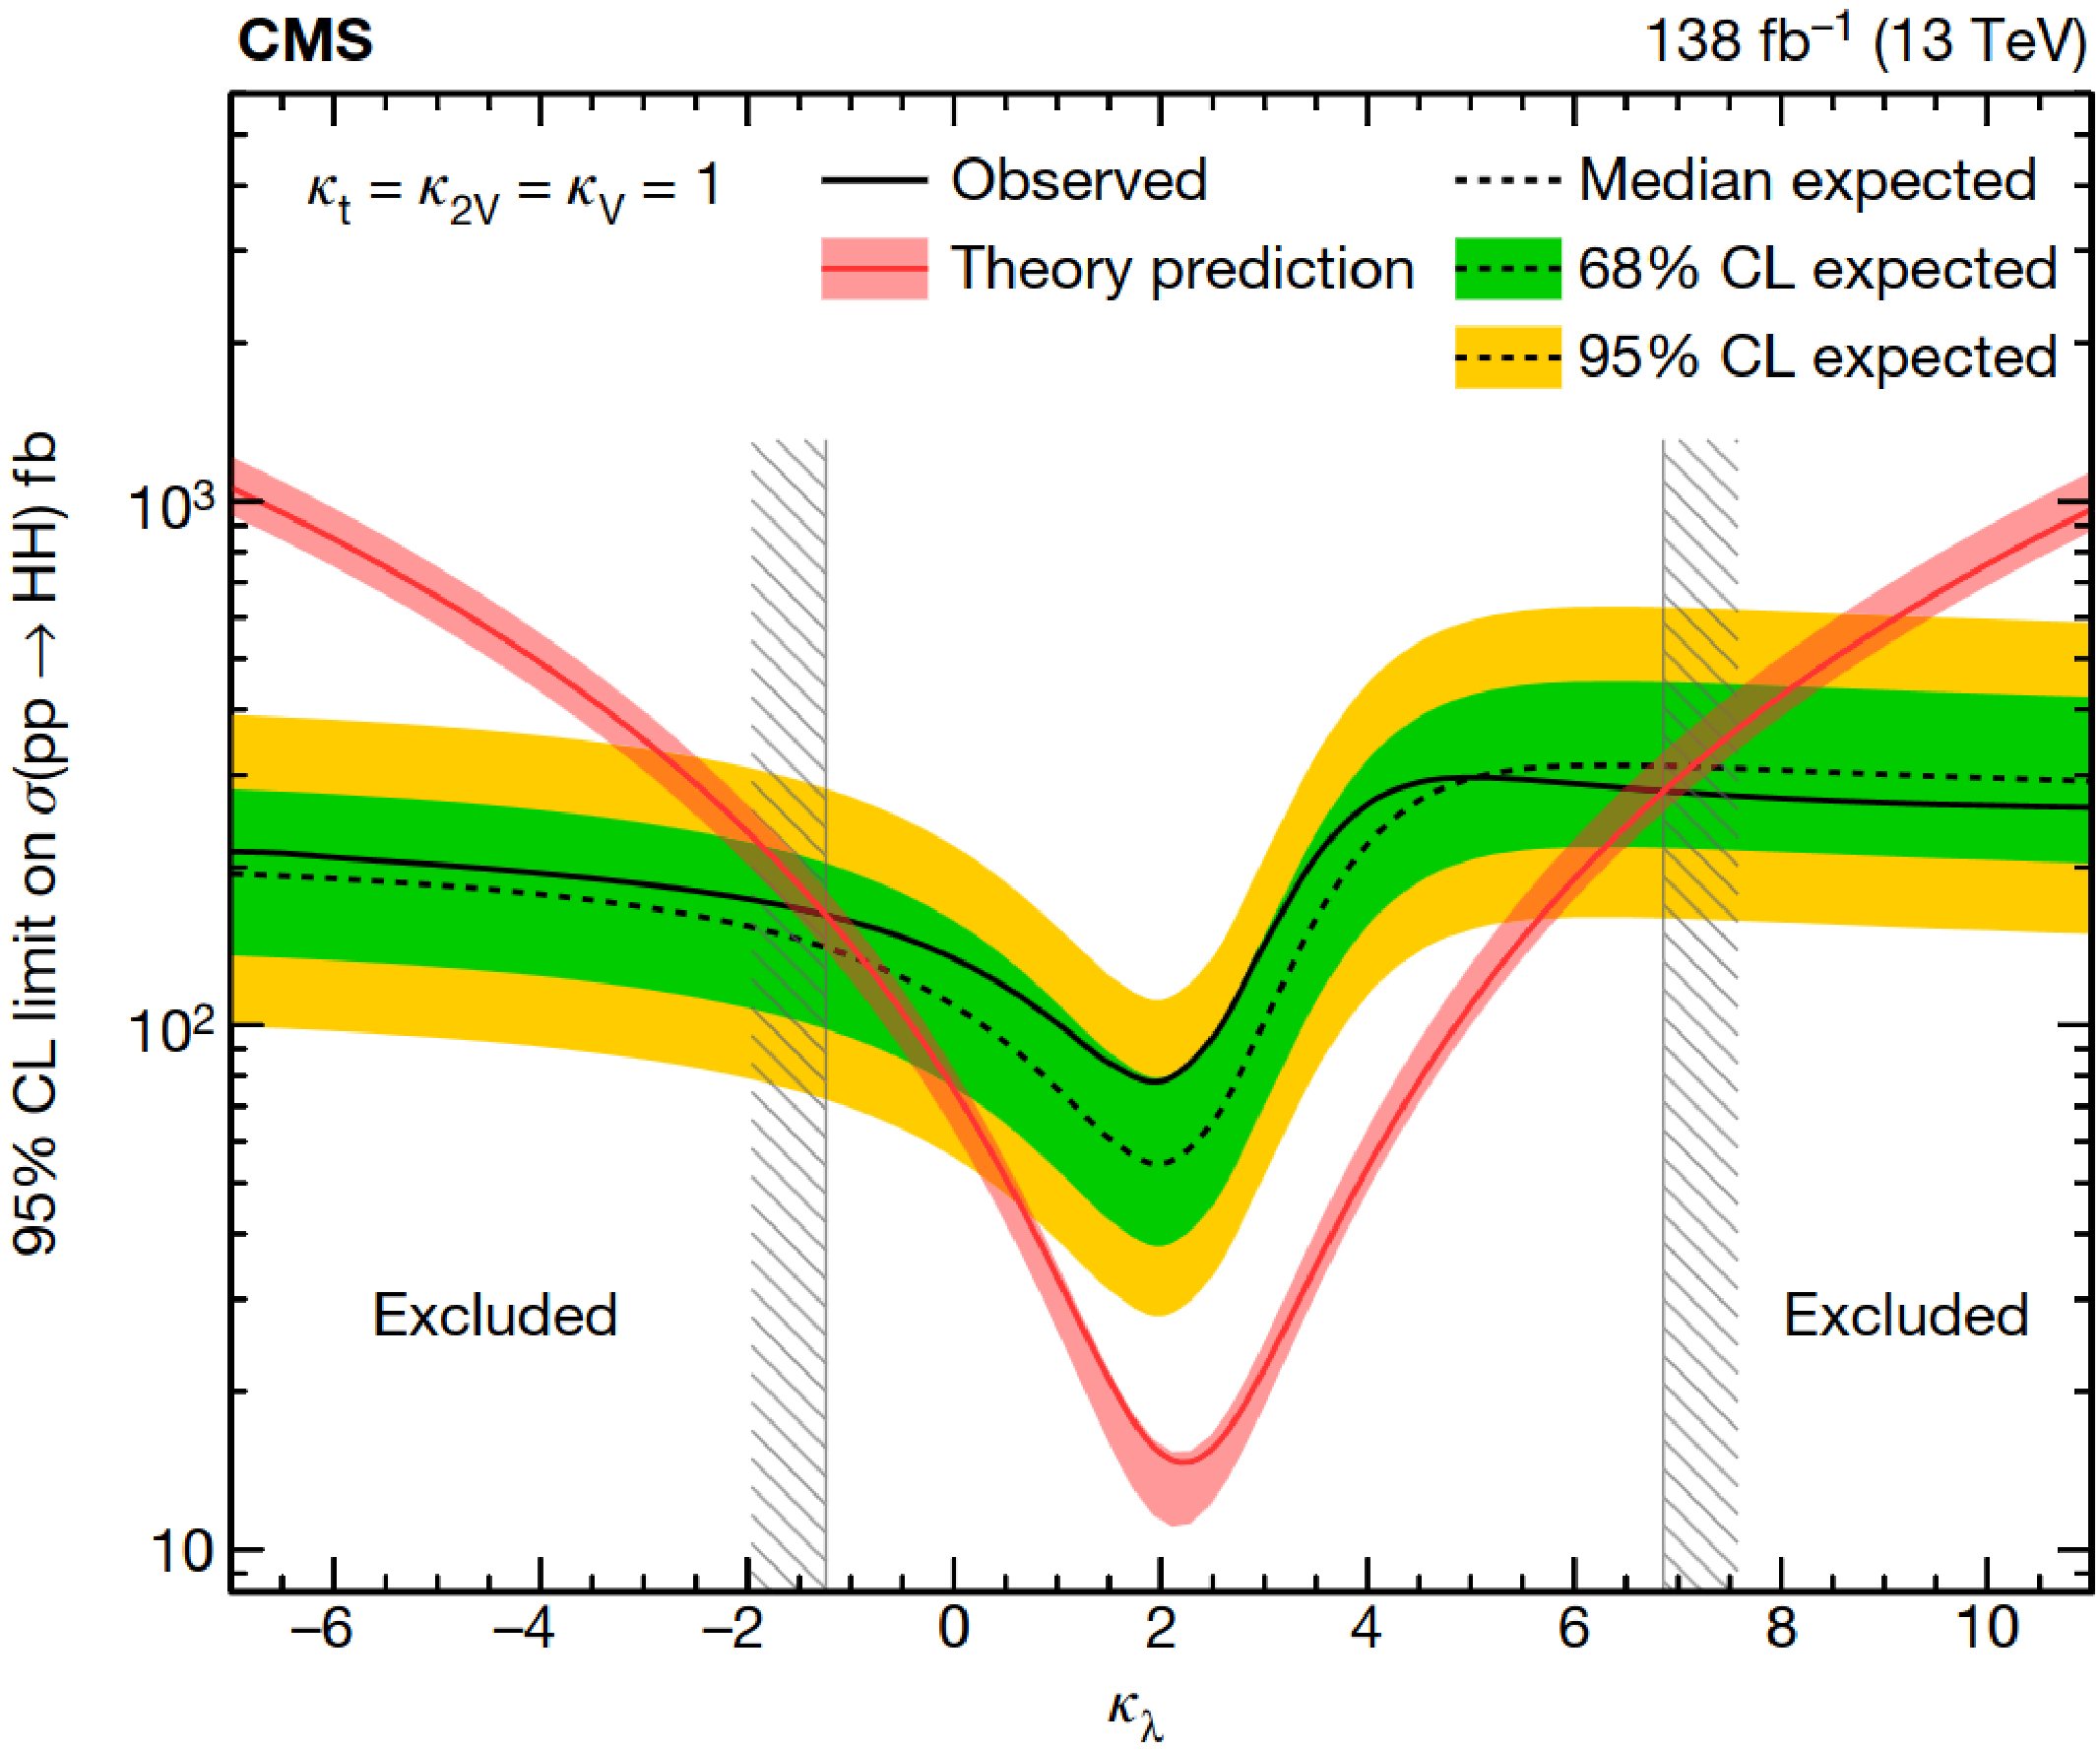
\includegraphics[width=.5\textwidth]{/home/bruno/org/PhD/Thesis/figures/scan_kl_nature.pdf}
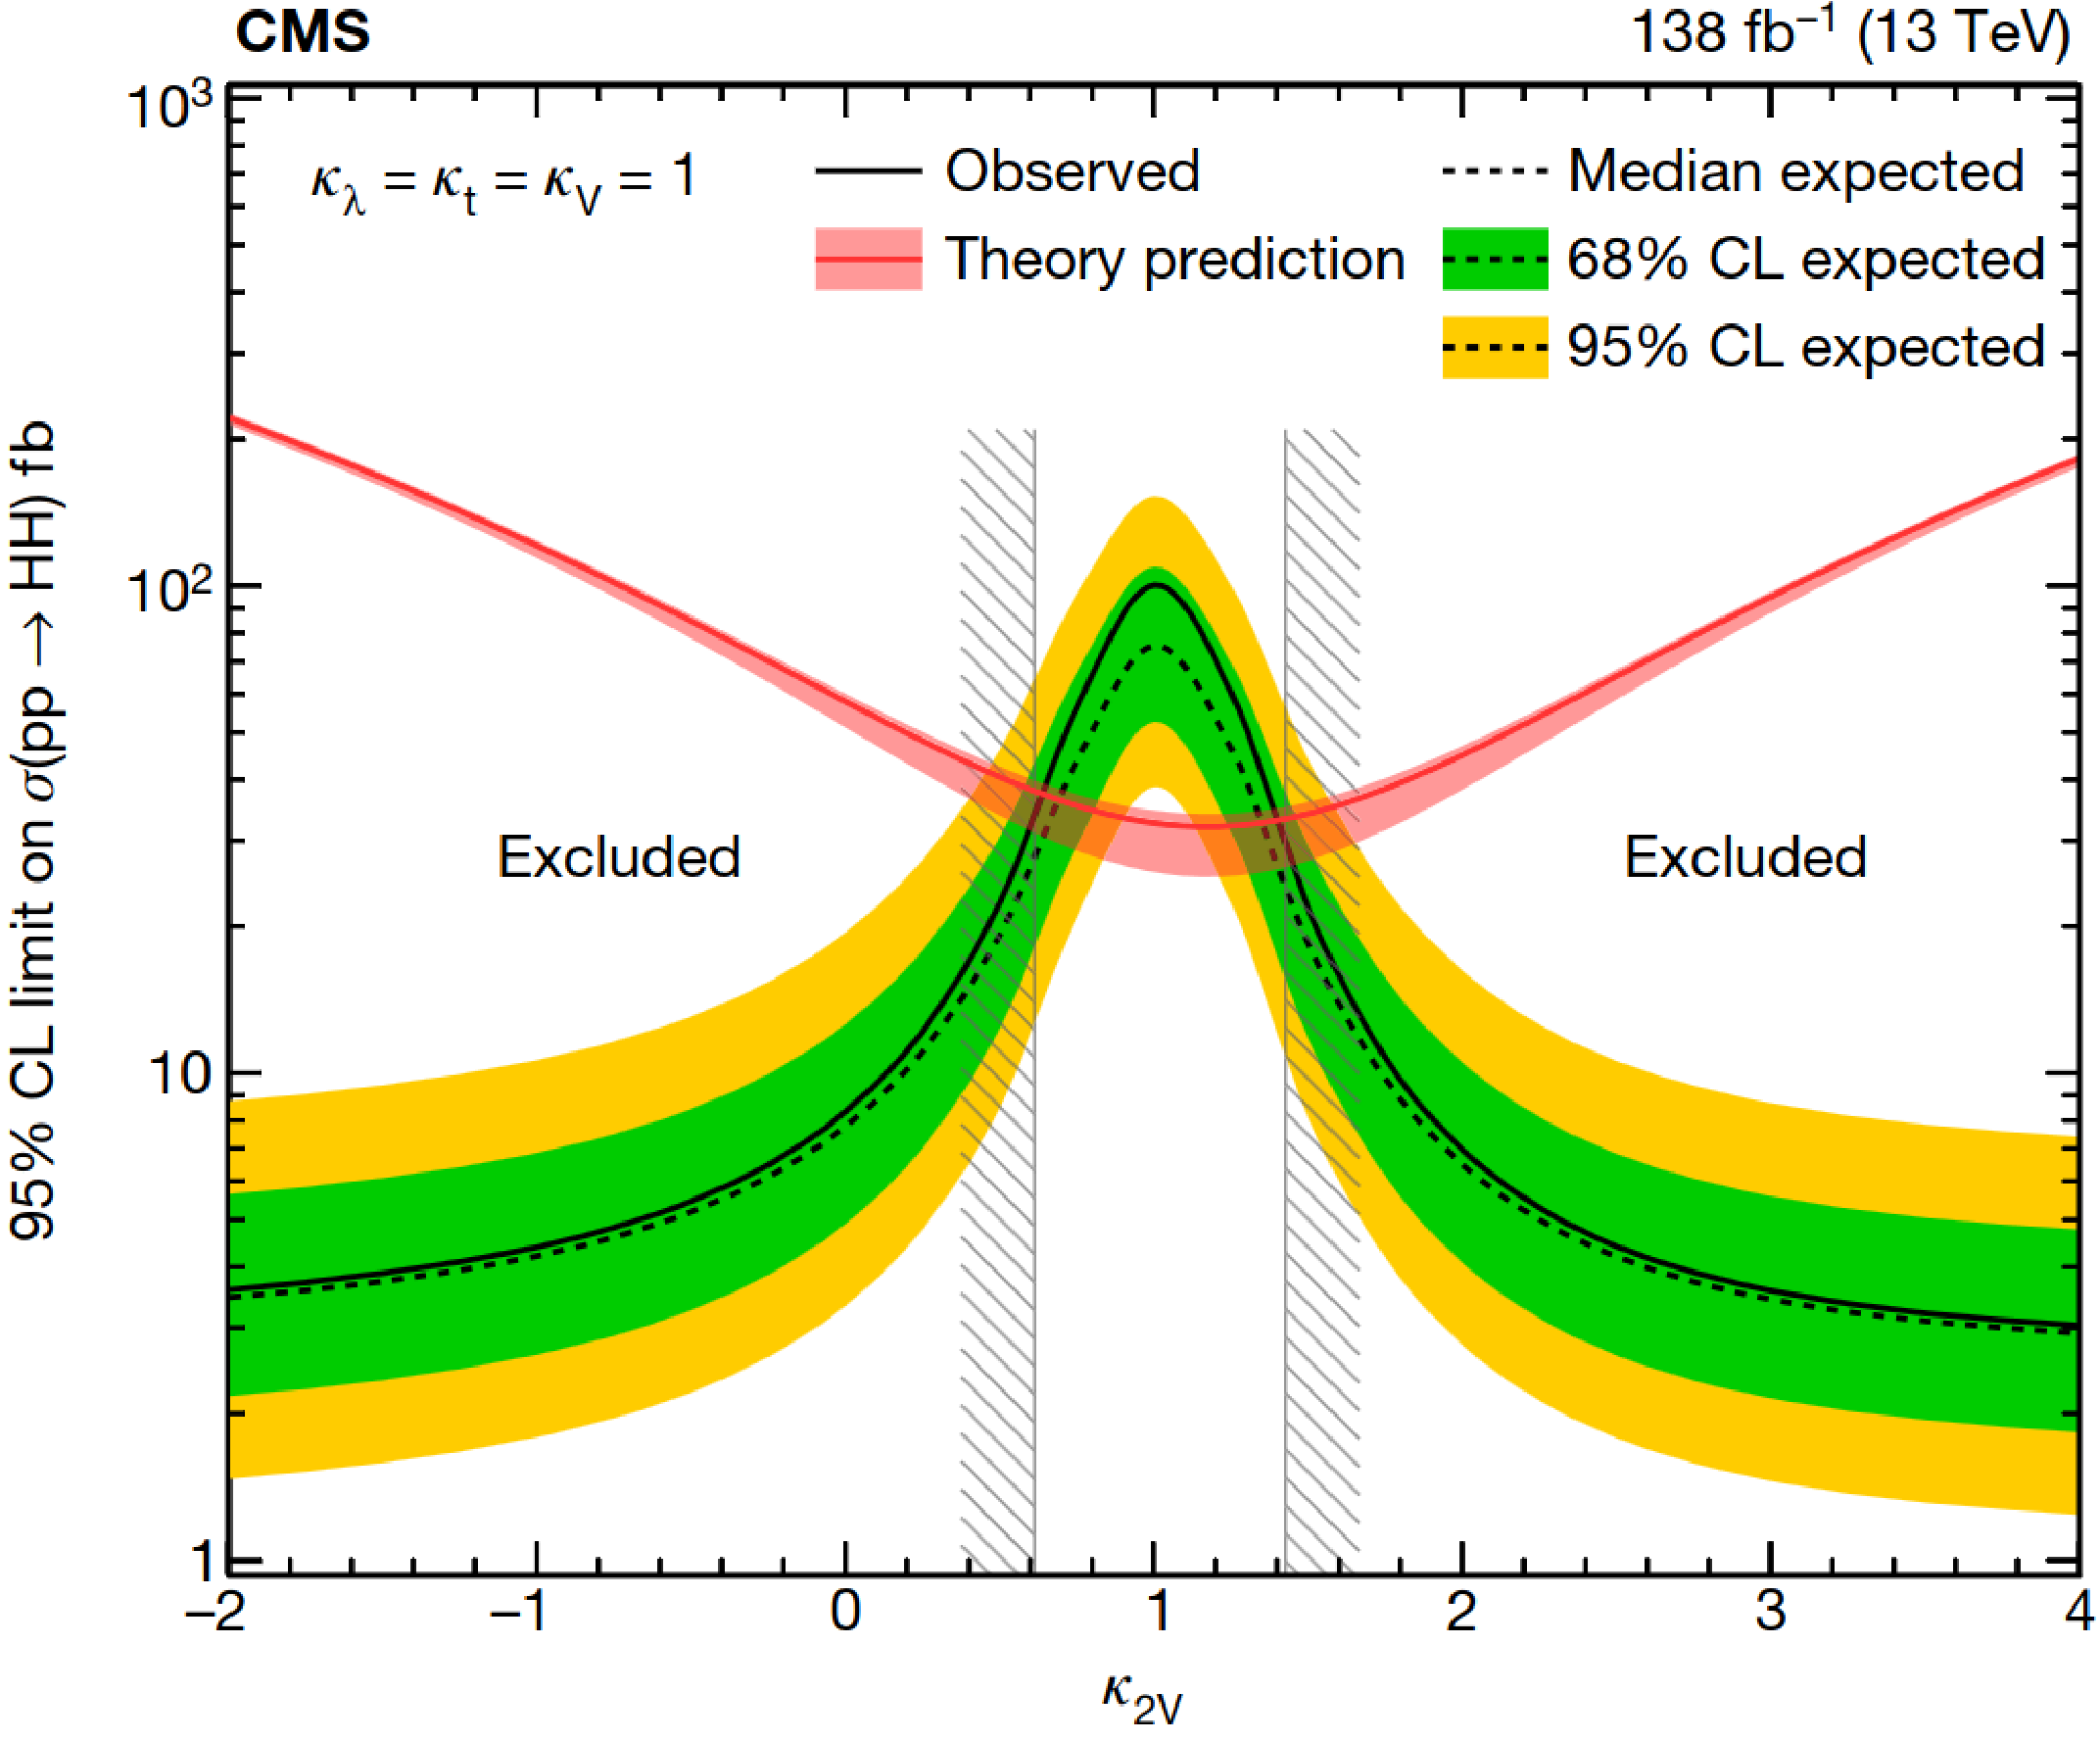
\includegraphics[width=.5\textwidth]{/home/bruno/org/PhD/Thesis/figures/scan_k2v_nature.pdf}
\caption{\label{org20bad4d}Combined expected and observed 95\% CL upper limits on the HH production cross-section for different values of \(\kl\) (left) and \(\kvv\) (right), assuming the SM values for other coupling modifiers. The green and yellow bands represent the 1\(\sigma\) and 2\(\sigma\) extensions beyond the expected limit, respectively; the red solid line (band) shows the theoretical prediction for the HH production cross-section (1\(\sigma\) uncertainty). The areas to the left and to the right of the hatched regions are excluded at the 95\% CL. Taken from \cite{higgs_10_years}.}
\end{figure}

\section{Recent nonresonant HH results}
\label{sec:org8a02e3e}
\subsection{\(\gamma \gamma \tau \tau\)}
\label{sec:orgb2ab82e}
\ac{CMS} has recently explored the extremely rare \(\gamma \gamma \tau \tau\) decay channel, for the first time, using full Run2 data.
The analysis covers non-resonant production via \ac{ggF} and the HH (spin 0 and 2) and HY \ac{BSM} resonant production modes.
The latter particle refers to an additional BSM scalar Y, considering both H(bb)Y(\(\tau \tau\)) and H(\(\tau \tau\))Y(bb) signatures.
Despite the minuscule HH branching ratio of 0.028\%, the analysis presents interesting specificities worth discussing.
In this work we focus on the nonresonant analysis only.

The analysis exploits di-\(\gamma\) triggers only, as triggering on the \(\tau\)'s is found to have a negligible impact.
Standard photon and lepton selections are applied.
The dominant backgrounds are peaking single-H and nonresonant \(\gamma\)+jets, \(\gamma \gamma\)+jets, \(\ttbar+\gamma\), \(\ttbar+\gamma\gamma\) and V\(\gamma\).
Minor backgrounds are taken from simulation.
The signal is fitted independently for different categories and data taking years with a double \ac{CB} function.
The background also includes a \hgg{} contribution which is modelled just like the signal.
The background continuum, instead, uses the discrete profiling method \cite{discrete_profiling}, which considers multiple analytical functions and penalizes functions with many parameters.

Interestingly, \(\tau\)’s are reconstructed in all its 6 decay modes (\(ee\), \(\mu\mu\), \(e\mu\), \(e\tau_{h}\), \(\mu\tau_{h}\) and \(\tau_{h}\tau_{h}\)), and additionally the single \(\tau_{h}\) and \(\tau_{h}+\text{track}\) channels are considered when no electorn or muon pass the selection.
Multiple selections are used, including a DY window mass veto to events compatible with \zll{} or \zllg{} close to the mass of the Z.

A \ac{BDT} is used, considering as input features related to the events' kinematical properties.
To avoid artificially creating a peaking structure in the di-\(\gamma\) mass (\(\mgg\)), which is used in the final fit, the \ac{BDT} is made independent of \(\mgg\) at first order.
This is achieved by not using \(\mgg\) as an input to the \ac{BDT} and by dividing the \(\pt\) of photon candidates by \(\mgg\).
Sequential boundaries are applied to the \ac{BDT}'s output to create two categories of different signal purities.
The splitting maximizes signal sensitivity.
Events not belonging to one of those two categories are discarded.

The final results are obtained performing a simultaneous maximum likelihood fit to \(\mgg\) in the two signal-enriched categories.
As expected by a SM behaviour, the analysis observed very few \(\gamma \gamma \tau \tau\) candidates.
However, it delivers observed (expected) \(\kl\) 95\% \ac{CL} upper limits, \(-13\;(-11) < k_{\lambda} < 18\;(16)\), and on the HH proton-proton cross-section, \(\sigma_{\text{HH}} < 930\;(740)\;\si{\femto\barn}\) or \(\sigma_{\text{HH}} < 33\;(26)\;\sigma_{\text{HH}}^{\text{SM}}\).
The limits are around one order of magnitude worse than the ones obtained by the most sensitive channels.

\begin{figure}
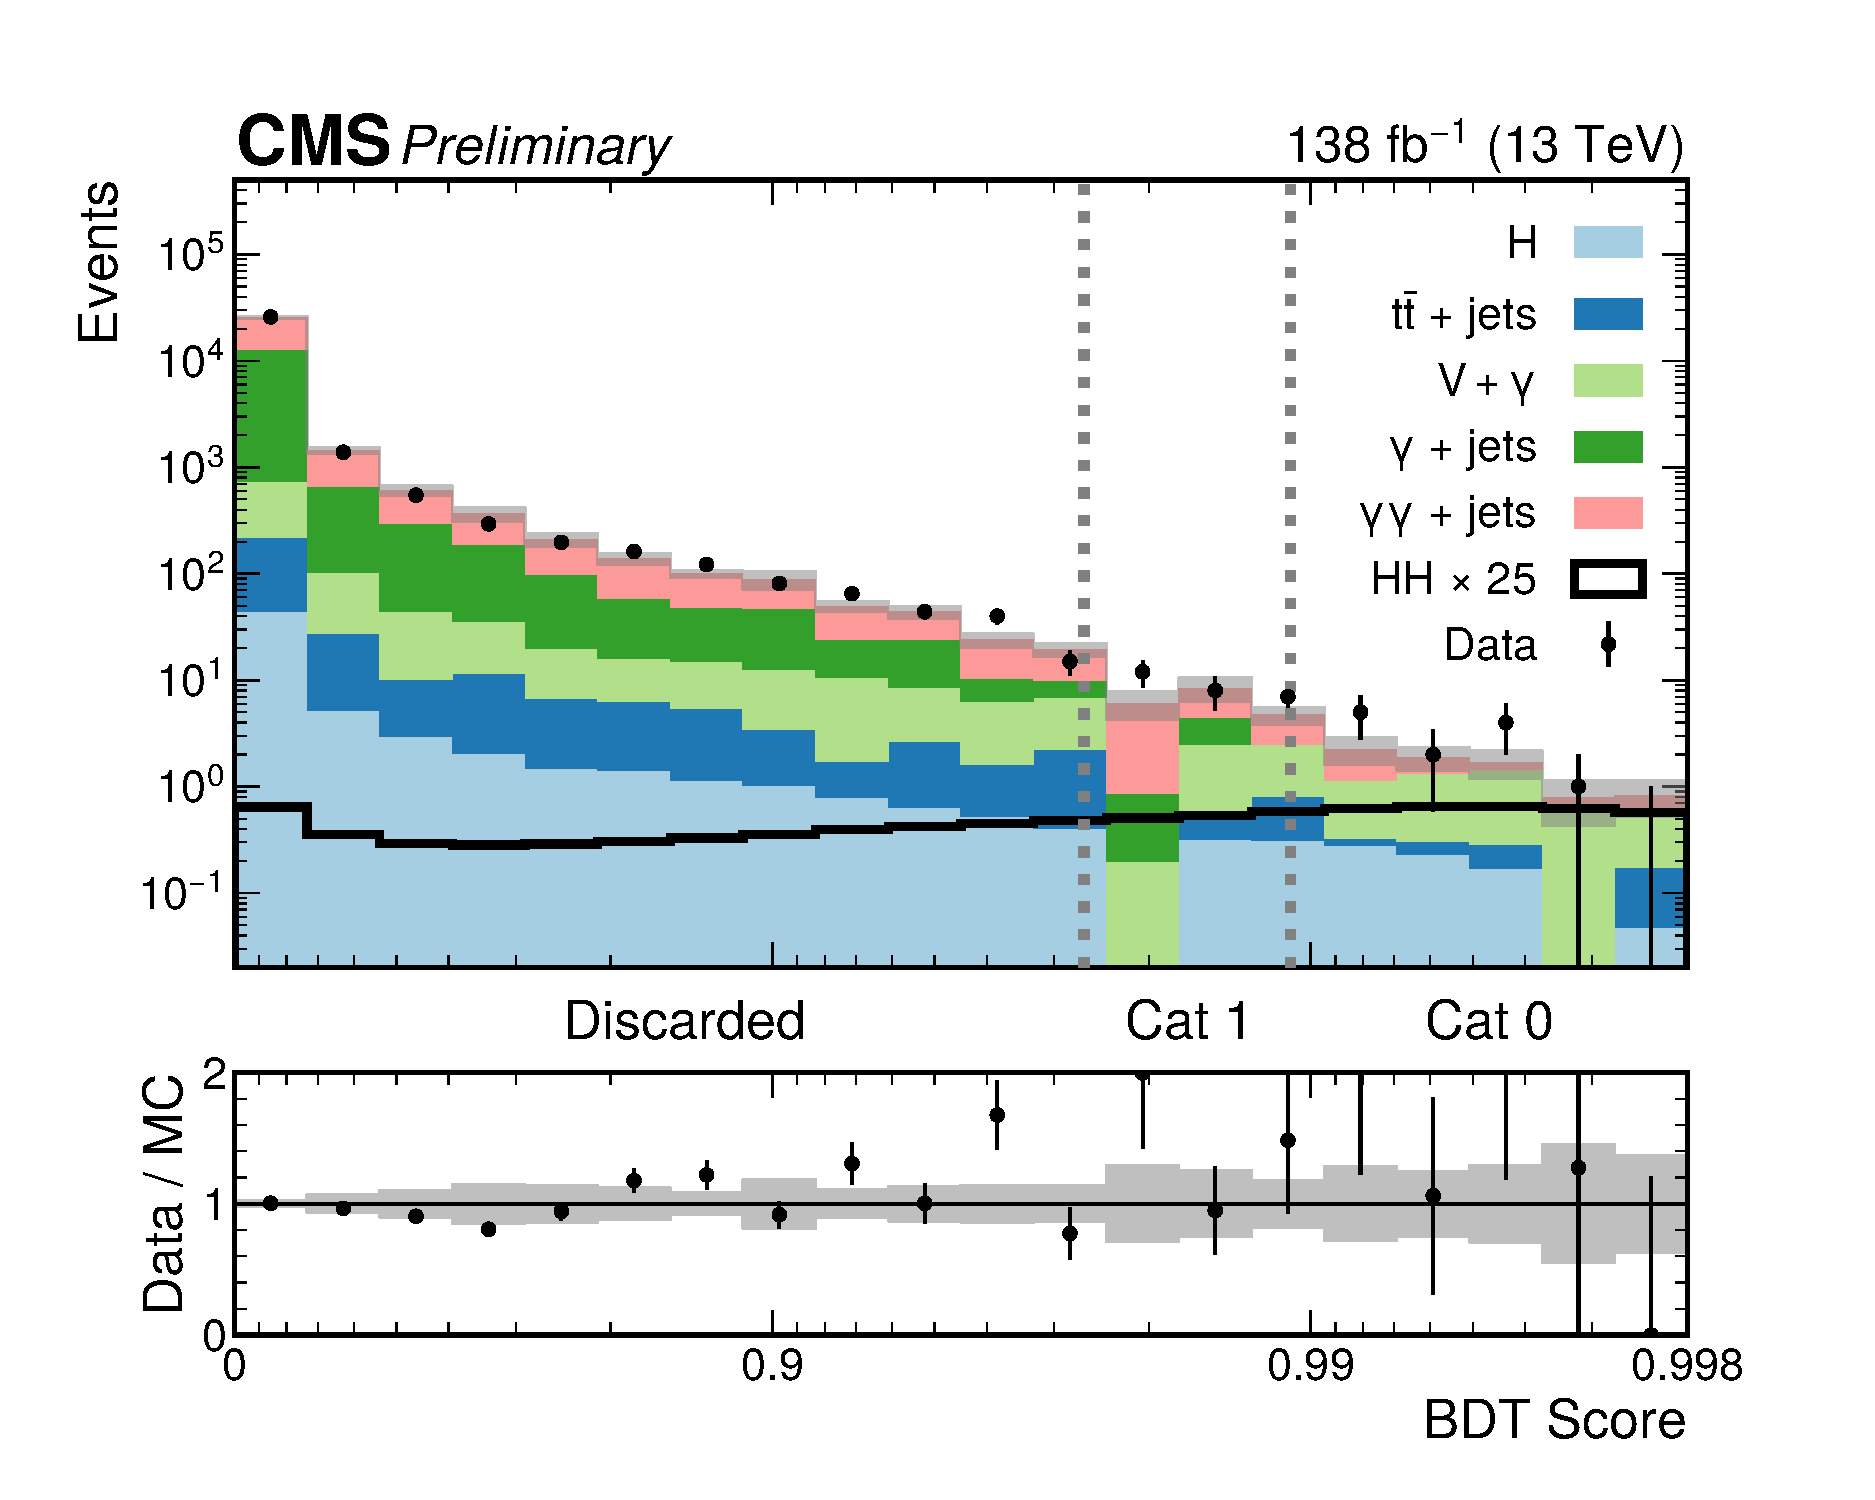
\includegraphics[width=.555\textwidth]{/home/bruno/org/PhD/Thesis/figures/ggtt_BDT.pdf}
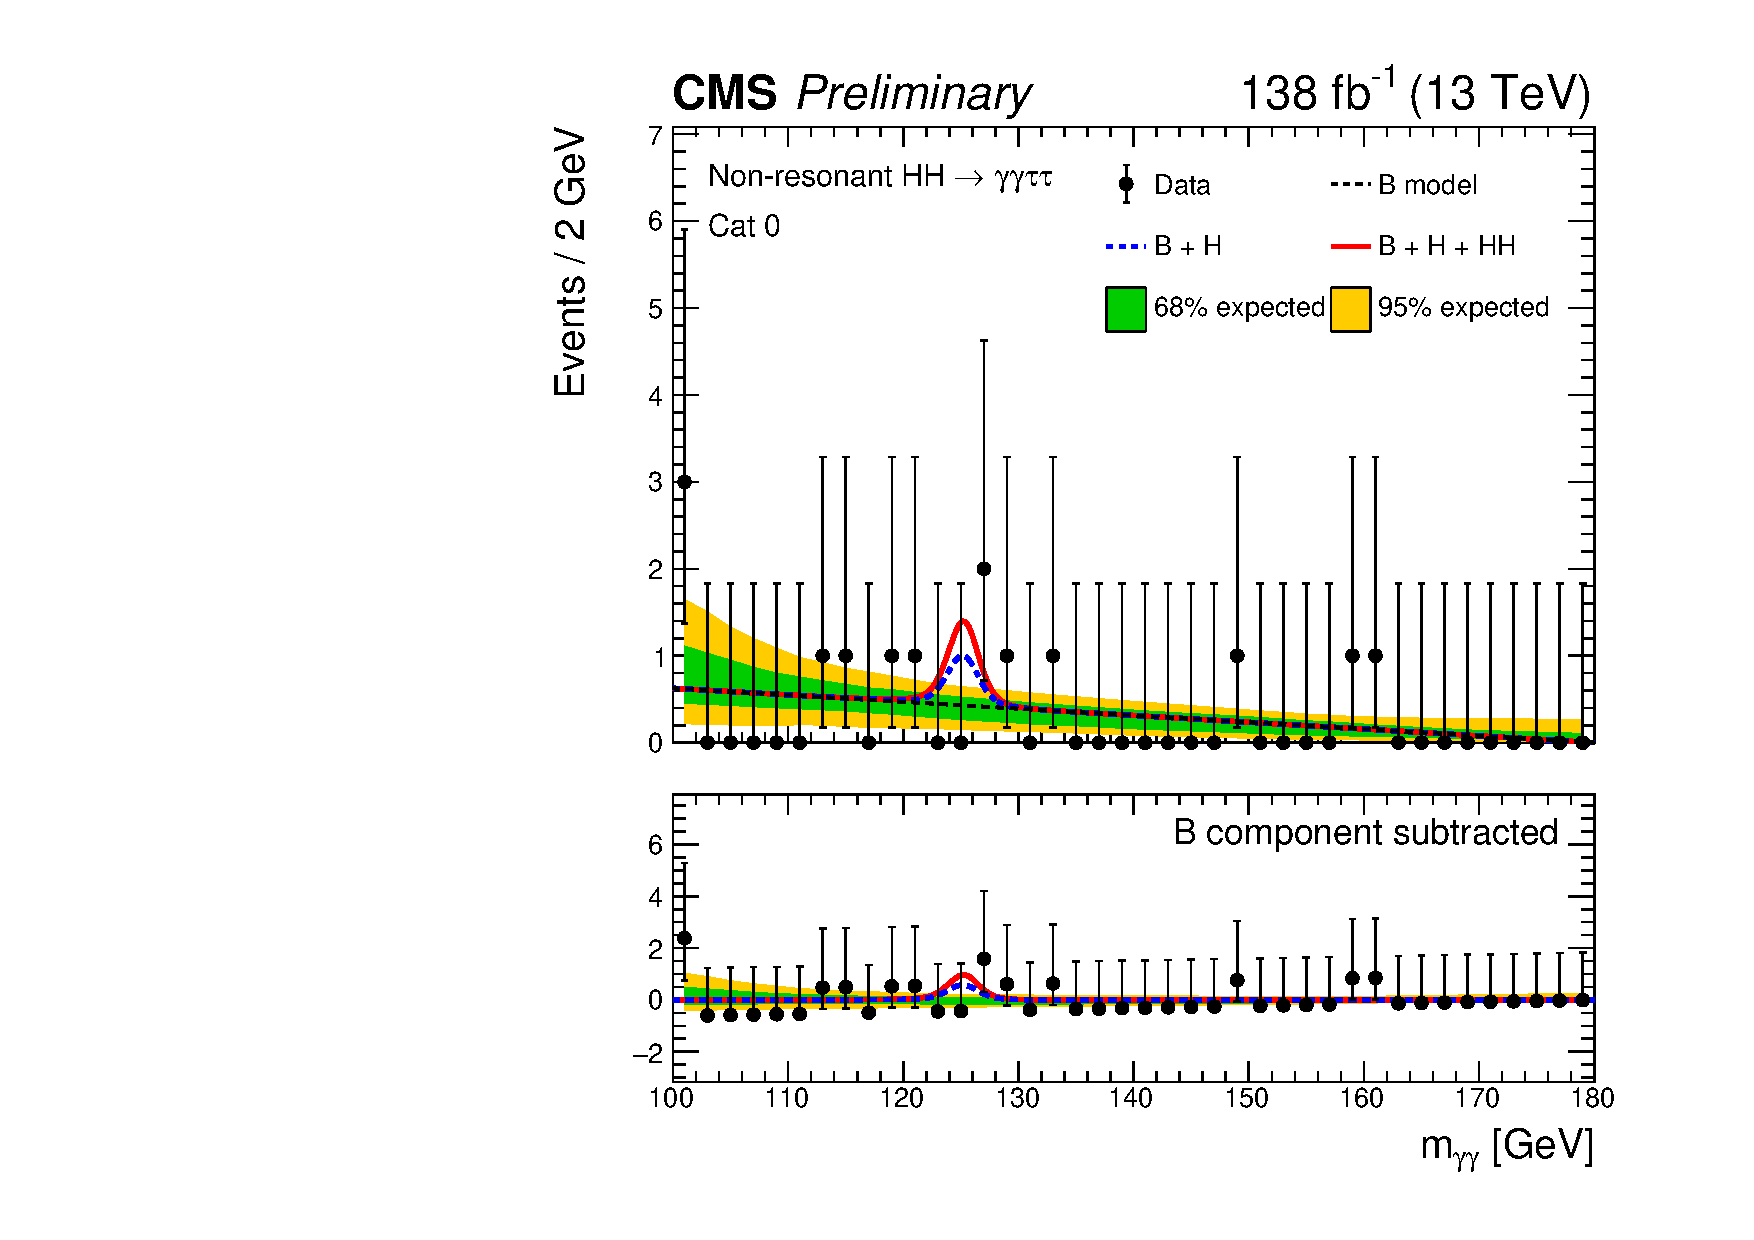
\includegraphics[width=.445\textwidth]{/home/bruno/org/PhD/Thesis/figures/ggtt_result.pdf}
\caption{\label{org93b6dfb}Results of the \(\gamma \gamma \tau \tau\) nonresonant analysis. \emph{Left)} Distribution of the BDT scores used for the event categorization from data and predictions from MC simulation. \emph{Right)} Data points and signal-plus-background models for the most sensitive analysis category, where the lower panel in each plot shows the residual signal yield after subtraction of the background. Taken from \cite{gammagammatautau}.}
\end{figure}
\subsection{Modelling the QCD background with the Hemisphere Mixing technique}
\label{sec:org71f7ef4}
\subsubsection{The \zzzhbbbb{} analysis}
\label{sec:orgacc05c1}
The ZZ and ZH processes represent standard candles to validate the HH analyses, given that they have cross-sections 31 and 8 times larger than the \ac{SM} ones, respectively, and are therefore expected to be observed before the \bbbb{} process.
The recently published resolved \zzzhbbbb{} analysis \cite{zz_zh_bbbb} uses a series of advanced background estimation techniques to successfully validate a \ac{QCD} estimate using synthetic datasets (\cref{orgd2c970a}).

In order to model the \ac{QCD} background, a control region is defined by requiring three b-tagged jets instead of four.
The dataset thus obtained, so as to reproduce the \ac{SR}, is weighted by two sets of weights, ti account for additional jet activity and subsisting kinematic mismatches.
The weights are derived in a di-jet mass sideband.

The analysis introduces a \ac{DNN} architecture especially designed to handle the b-quark pairing combinatorics: the \ac{HCR} network.
A detailed explanation is outside the scope of this work, but suffices to say that it is used to discriminate signal from background, to define the background model kinematic weights, and to differentiate \ac{QCD} from \(\ttbar{}\) in the technique of \cref{orga77051f}.

The final fit is validated using the synthetic dataset, without statistical fluctuations, and using one of the mixed models as the four-tag data. Systematics behaved as expected and the result was compatible with a zero signal strength.
The observed (expected) 95\% CL upper limits on the production cross sections correspond to 3.8 (3.8) and 5.0 (2.9) times the \ac{SM} prediction, for the \zzbbbb{} and \zhbbbb{} processes, respectively.
The analysis indicates that ZH will likely be ovserved first.

\subsubsection{The problem with \ac{QCD} simulations}
\label{sec:org736a79b}
\label{orgd2c970a}

Many analysis in CMS include quark- or gluon- induced jets in their final state particles.
This is also the case for some HH analysis, including the most sensitive ones (since they include a pair of b-jets) \cite{higgs_bbtautau_nonres,bbgg_cms,bbbb_resolved_cms,bbbb_boosted_cms}.
\ac{QCD} backgrounds are often significant, and sometimes dominant, as in \bbbb{} analysis, where the second most common source of background, \(\ttbar\), is almost an order of magnitude less common.
Unfortunately, currently available \ac{QCD} simulations lack the required precision and statistics for a robust background estimate, particulary in the higher energy distribution tails.

Data-driven methods are therefore usually employed to model the \ac{QCD} background.
These usualy take the form of ``ABCD-like'' methods, where \acp{CR} are defined in such a way as to ensure orthogonality with respect to the \ac{SR}.
Some variants exist, such as (possibly high-dimensional) ``alphabet'' \cite{corcodilos_thesis} and ``fake factor'' \cite{fake_factor_method,higgs_bbtautau_hy} methods, but the general principles, especially in the context of this work, are similar.
The basic idea is to find fully uncorrelated variables upon which the \ac{SR} selection depends on, and invert the cuts to obtain signal-free regions.
The latter can be used to estimate both the shape and the normalization of the \ac{QCD} background in the \ac{SR}, without using it directly.

To give an example, in the most recent \bbtt{} non-resonant analysis \cite{higgs_bbtautau_nonres}, the \(\tau\) isolation and the relative sign of the charges of the two leptons are used to create three \acp{CR} around the analysis \ac{SR} (opposite-charged leptons and well isolated \(\tau\)'s). Defining B, C and D as three \acp{CR} where B has equally charged leptons and tight isolation, C has opposite charged leptons and loose isolation, and D has both cuts inverted, the shape of the \ac{SR} can be inferred either by B or C and the normalization by B/D or C/D, respectively.
In the resolved \bbbb{} analysis \cite{bbbb_resolved_cms}, instead, the control regions are defined based on the invariant mass of the two Higgses and on the number of b-tagged jets.
The \ac{SR}, having 4 b-jets, has its \ac{QCD} background modeled from events in \acp{CR} with 3-bjets.
It is assumed that kinematic properties are similar between \acp{CR} and the \ac{SR}. 

In all cases, the background is derived in a signal-free region, and thus requires an extrapolation to a different region of the phase-space.
In order to validate the extrapolation, a \ac{VR} is usually employed.
However, the definition of an additional region will necessarily deplete the signal region.
Additionally, the extrapolation cannot be directly tested, since the \ac{VR} differs from the signal region inasmuch as it will not be signal-enriched.
Finally, both \acp{CR} and \acp{VR} often have low statistics, and become a dominant source of systematic uncertainties.
Indeed, finite data in \acp{VR} imply an ``inherent limitation on the capability to validate the performance of the background model'' \cite{zz_zh_bbbb}.
There is therefore a need to develop new methods to estimate and validate the \ac{QCD} background estimation that are not sensitive to low statistics.
In addition, it would be beneficial to directly test the ABCD extrapolation in the \ac{SR}.


\subsubsection{Hemisphere mixing}
\label{sec:org8eb1abc}
\label{orga77051f}

The hemisphere mixing technique \cite{hemisphere_mixing} first creates a library of ``hemispheres'', which arise from the splitting of events along the plane orthogonal to the transverse thrust axis.
The latter is in turn defined as the axis where the sum of the absolute values of the \(\pt\) projections of the all the jets in the event is maximal.
The splitting is done using a sample of events with four b-tagged jets, thus ``pure'' in signal events.
For each hemisphere a set of four variables is calculated: mass, longitudinal momentum, and transverse momentum perpendicular and parallel to the thrust axis.
A second pass on data mixes pairs of hemispheres by minimizing the distance of two hemispheres in terms of a normalized sum of the summary variables.
The two hemispheres must belong to different events.

The paper here discussed \cite{zz_zh_bbbb} contributes with two improvements to the original hemisphere mixing technique.
Firstly, the mixing step is performed with 3-tagged data in order to increase statistics and make (4-tagged) signal contamination negligible.
Statistics are also increased by lowering the b-tag \ac{WP} used on the three jets.
Secondly, the non-negligible presence of \(\ttbar{}\) events is mitigated by removing such events from the mixing stage.
This is done event-by-event via a classification with the \ac{HCR} network, which calculates the probability P(M) for each event to be multijet, where a random number X is generated between 0 and 1. If \(\text{X} > \text{P(M)}\), the event is rejected.

For the validation of the background model, we have to ensure the size of the synthetic dataset is comparable to the one used for the model.
The hemisphere dataset is thus sub-sampled, and 15 separate mixed models are formed, given the available statistics.
Systematic uncertainties of the \ac{QCD} modeling are determined using the synthetic dataset in three different ways:
\begin{enumerate}
\item Differences between mixed models, arising from limited statistics, are quantified by using their average;
\item The background model is compared with the mixed models in the signal region;
\item An unconstrained signal template is added to the signal + background fit to verify if a spurious signal can be mimicked by the background model. This fit is compared with a background-only fit and found to be in agreement.
\end{enumerate}

Importantly, and despite not yet being used in the most recent \bbbb{} results, a principled and precise way of measuring the most important systematics directly in the \ac{SR} is now available.
We note that, given appropirate modifications, a similar method could be extended to the \bbtt{} analysis.
\subsection{Single and double Higgs combination}
\label{sec:orgdbd6425}
\label{org9913bdc}

On top of the HH searches already mentioned, \(\kl\) can be additionally constrained by exploiting \ac{NLO} \ac{EW} corrections to single Higgs processes, which also depend on \(\kl\).
Single Higgs cross-sections can indeed be quite sensitive to \(\kl\) variations, especially in the VH and ttH production modes, where up to 10\% differences are expected.
Additionally, there is a strong complementarity between direct and indirect searches.
HH searches generally provide weaker contraints on the Higgs boson coupling to fermions and vector bosons, due to the lower production cross-section with respect to single Higgs.
On the other hand, double Higgs processes provide stronger constraints on \(\kl\).

The main challenge of the combination recently performed by \ac{CMS} \cite{CMSHplusHHcomb} consists on estimating and efficiently removing overlaps between signal regions of different analysis.
The mitigation of double-counting and minimization of overlaps, together with the combination of event categories from both single and double-Higgs analysis, lead to stronger \(\kl\) constraints.
The analysis with the most sensitive production modes are included.
Whenever overlaps exist, one of two approaches is taken: either additional selections are applied, or the least sensitive category or analysis is removed.
As an example, the \bbzz{} analysis is removed in favour of \zzfourl{} due to the former's relatively low sensitivity to \(\kl\).
Concerning systematics, their modelling in HH processes is generally simpler when compared to single H, due to the limited statistics of HH.

\ac{CMS} observed exclusion intervals at 95\% \ac{CL} of \(-0.4 < \kl < 6.3\), assuming other Higgs couplings to follow the \ac{SM}, or \(-1.4 < k_{\lambda} < 6.1\) otherwise.
For comparison, \ac{ATLAS} observed \(-0.4 < \kl < 6.3\), assuming \ac{SM} couplings, or \(-1.4 < k_{\lambda} < 6.1\) otherwise \cite{ATLASHplusHHcomb}.
We show (\(\kl\), \(\kt\)) and (\(\kv\), \(\kvv\)) scans in \cref{orga6f270a}, where the complementarity between the two types of processes is clearly highlighted.
\ac{CMS} was also able to once again \cite{higgs_10_years} exclude \(\kvv=0\) at more than 5\(\sigma\), this time without fixing \(\kv=1\).

\begin{figure}
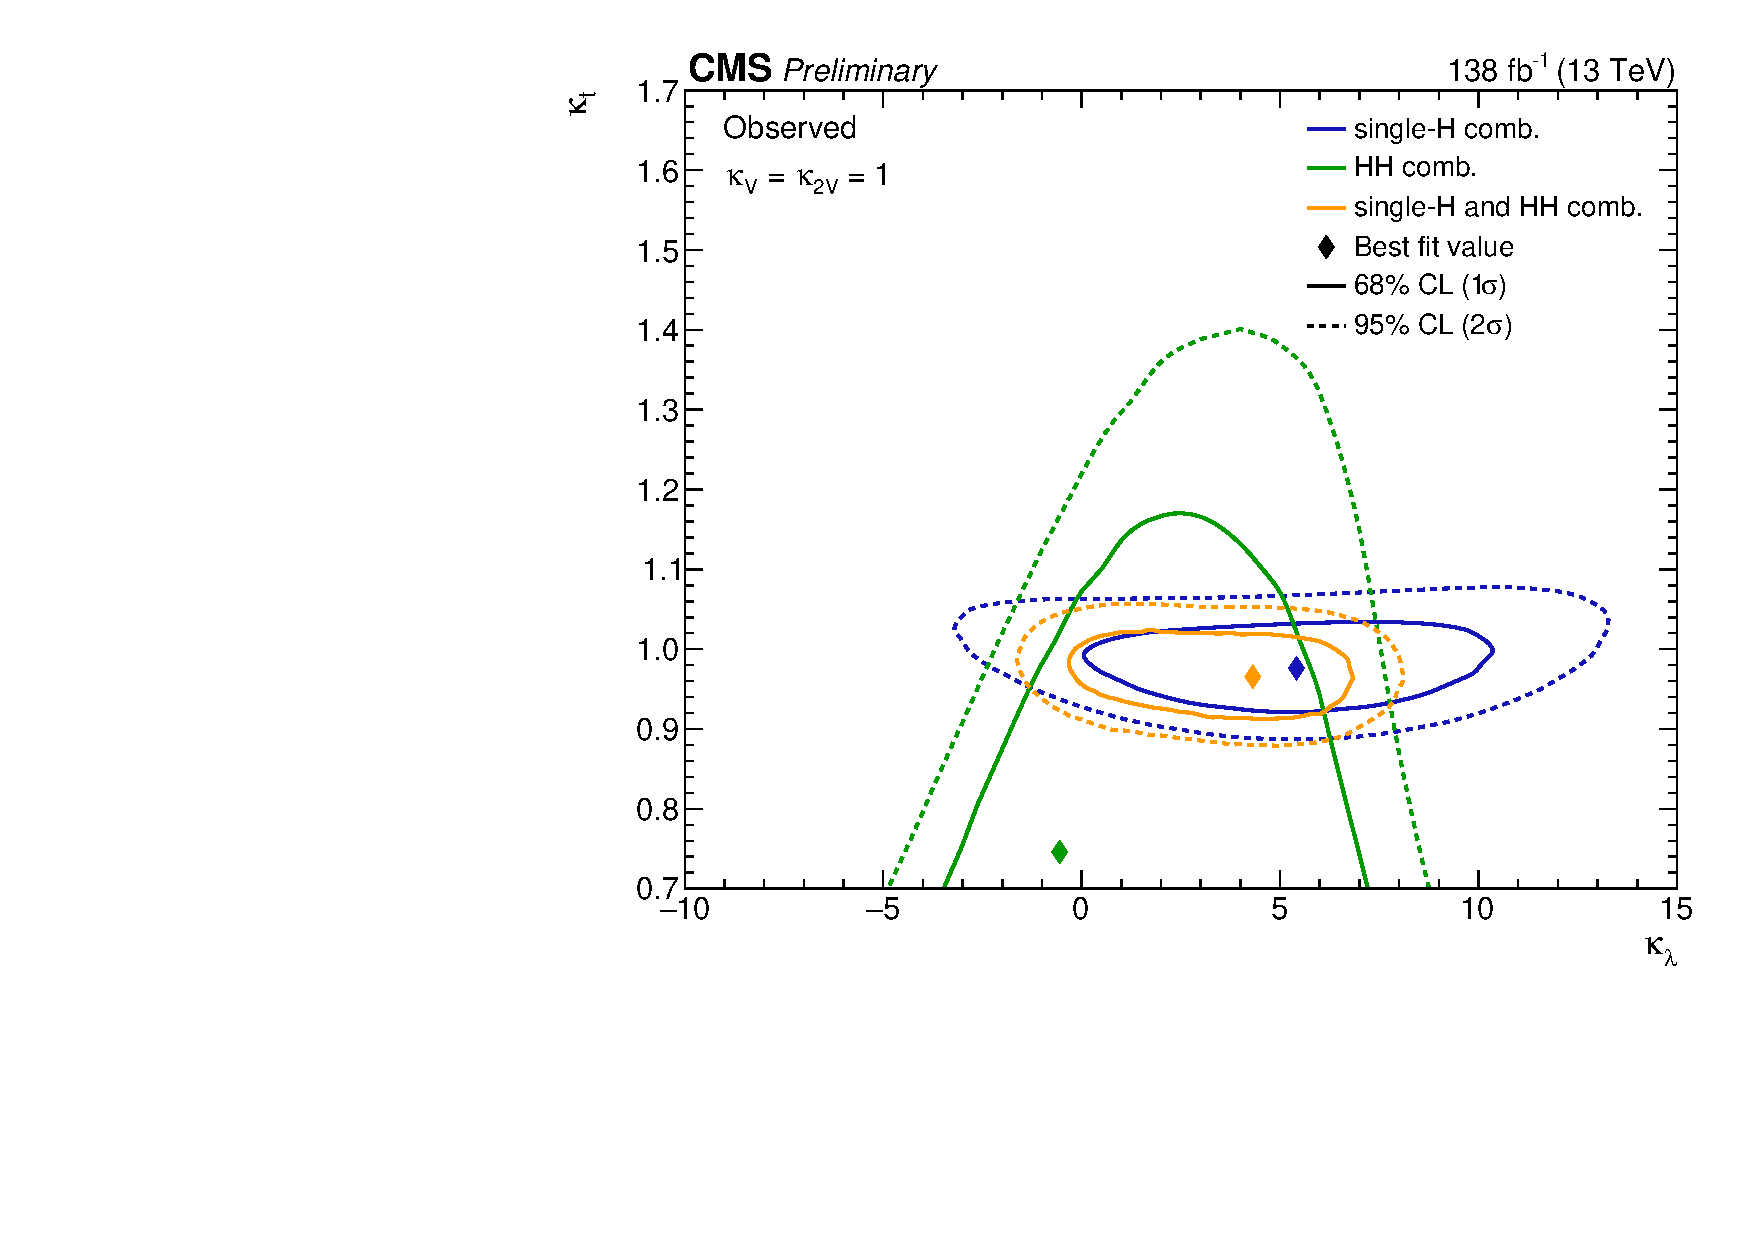
\includegraphics[width=.5\textwidth]{/home/bruno/org/PhD/Thesis/figures/combination_single_double_kl_kt.pdf}
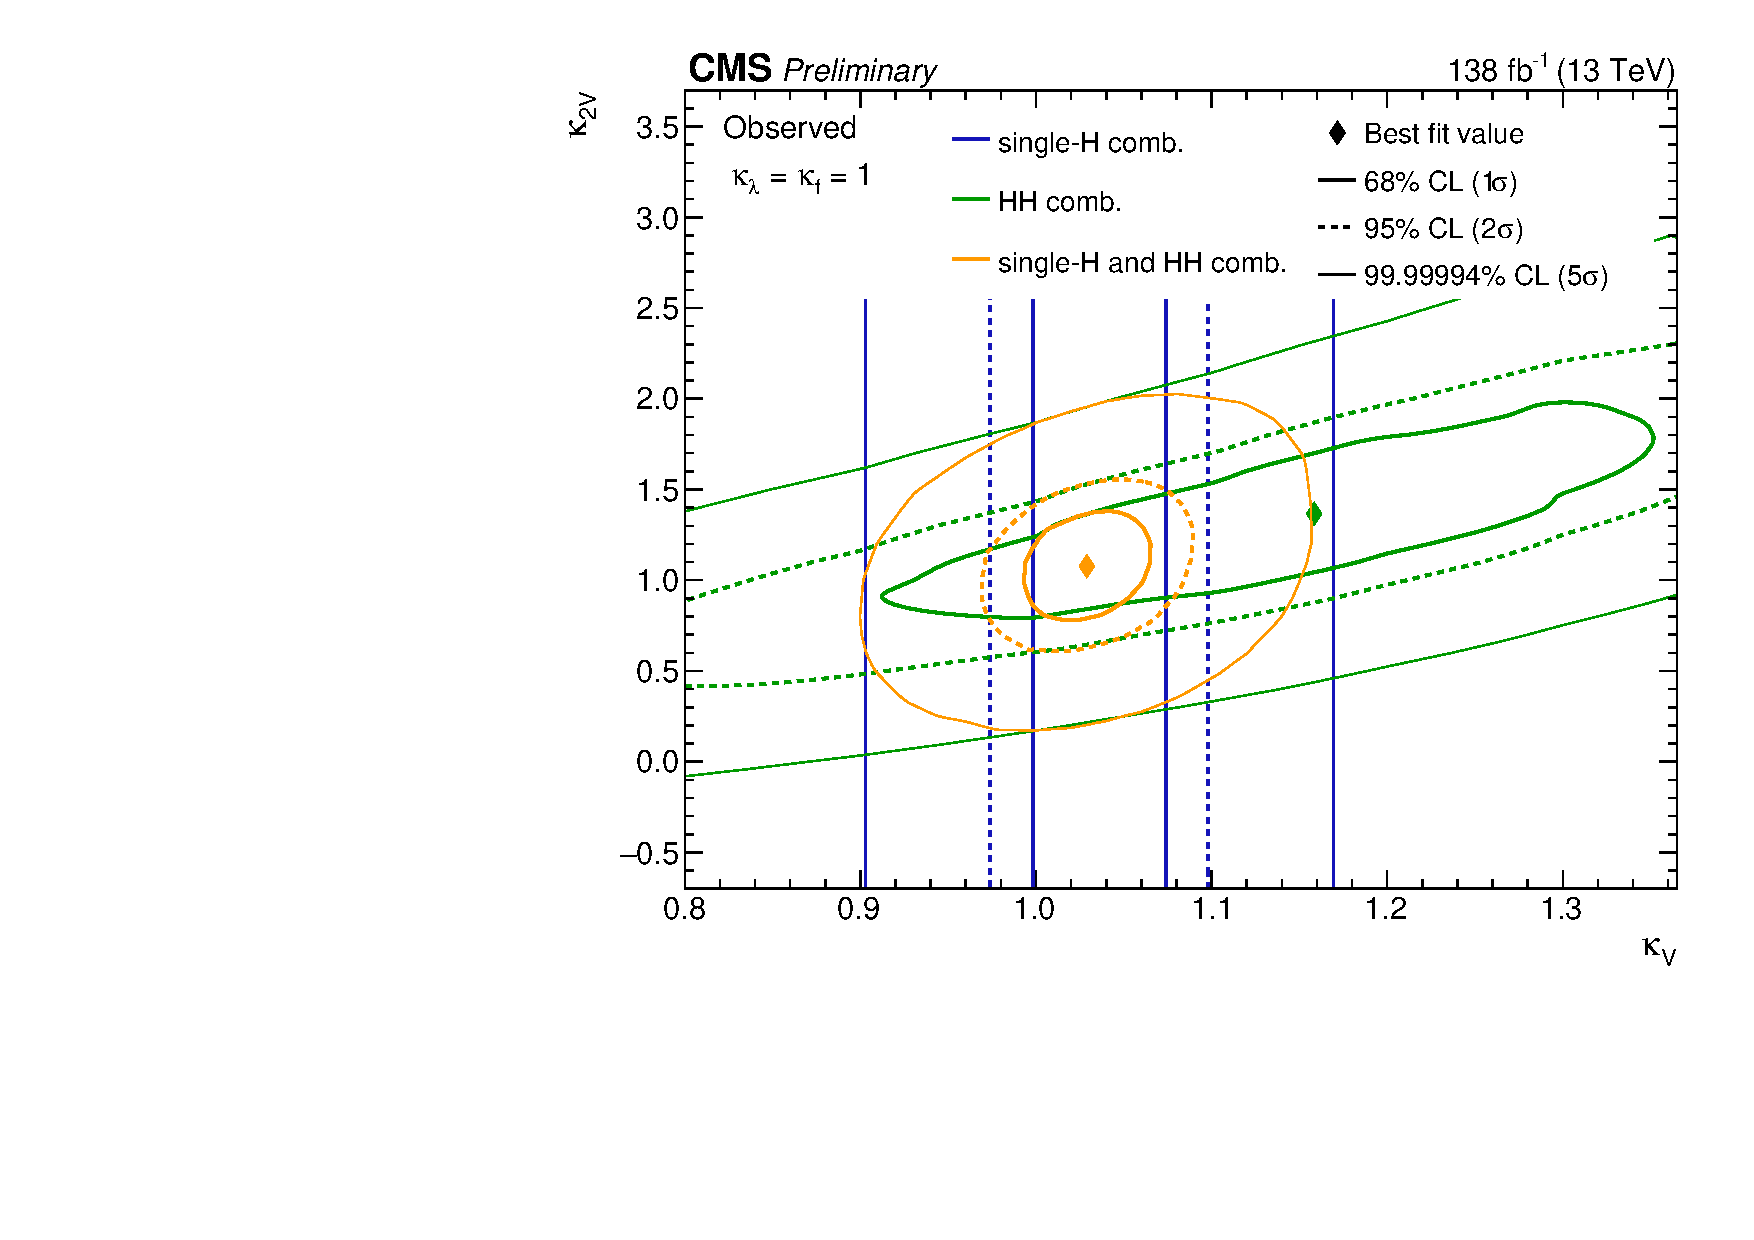
\includegraphics[width=.5\textwidth]{/home/bruno/org/PhD/Thesis/figures/combination_single_double_k2v_kv.pdf}
\caption{\label{orga6f270a}Observed two-dimensional likelihood scans of (\(\kl\), \(\kt\)) (left) and (\(\kv\), \(\kvv\)) (right). The strong complementarity between the single and double Higgs processes is well illustrated. The remaining coupling modifiers are set to their \ac{SM} value. Taken from \cite{CMSHplusHHcomb}.}
\end{figure}

\section{Run 3 and beyond}
\label{sec:org082b4f4}
\label{org67f6d26}

The near future promises further constraints on \(\kl\) and on \ac{EFT} couplings in the context of nonresonant HH searches.
Yet unexplored HH production modes and decay channels are currently being studied.
On top of the recent \(\kvv=0\) exclusion, and assuming \(\kl=1\), we hope to measure nonresonant HH via a multi-channel combination by the end of the \ac{HL-LHC} \cite{higgs_10_years}.
Uncertainties are still dominated by the lack of statistics, but \ac{ggF} theory uncertainties might become important in the future.

For the moment, Run3 is an opportunity to bring improvements before the start of the \ac{HL-LHC}.
New techniques, including better estimates of \ac{QCD} background and new machine learning methods, will make existing results quickly obsolete.
The usage of \ac{PNet} \cite{particle_net} for \(\tau\)-initiated jets and the application of transformer technology to jet tagging \cite{particle_transformer} might have a strong impact.
Additionally, an improved trigger strategy has been implemented, considering both data scouting and parking \cite{parking_scouting_run3_cms}, and with the inclusion of \ac{PNet} b-tagging directly in the trigger.
The inclusion of \ac{PNet} \(\tau\)-tagging at trigger level is being envisaged, and might be done still during Run3.
We also expect that some HH analysis might benefit from the inclusion of synthetic datasets, as discussed in \cref{orga77051f}.
The first \ac{CMS} Run3 HH results will soon be available.

\bibliographystyle{unsrt}
\bibliography{../../../dot-emacs/bibliography/references/higgs,../../../dot-emacs/bibliography/references/l1,../../../dot-emacs/bibliography/references/hgcal,../../../dot-emacs/bibliography/references/mc_generation}
\end{document}
